4. \begin{figure}[ht!]
\center{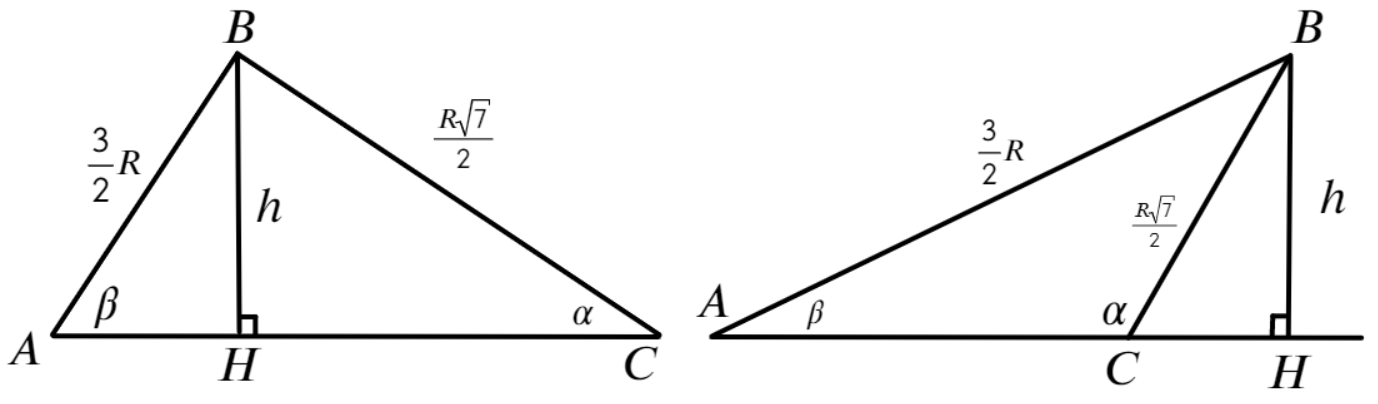
\includegraphics[scale=0.35]{g9-4.png}}
\end{figure}\\
По теореме синусов $\cfrac{\cfrac{3}{2}R}{\sin(\alpha)}=\cfrac{R\cfrac{\sqrt{7}}{2}}{\sin(\beta)}=2R,$ значит $\sin(\alpha)=\cfrac{3}{4},\ \sin(\beta)=\cfrac{\sqrt{7}}{4}.$ Так как $\cfrac{3}{2}>\cfrac{\sqrt{7}}{2},\ \alpha>\beta,$ поэтому тупым может быть только угол $\alpha$ (если угол $\beta$ является тупым, то сумма углов треугольника больше $180^\circ.$)Опустим высоту из точки $B,$ тогда $h=\cfrac{3}{2}R \sin(\beta)=\cfrac{3\sqrt{7}}{8}R.$ Возможны два случае: точка $H$ лежит на стороне $AC$ или вне её. В первом случае $AC=AH+HC=\cfrac{3}{2}R \cos(\beta)+R\cfrac{\sqrt{7}}{2}\cos(\alpha)=
\cfrac{3}{2}R \sqrt{1-\cfrac{7}{16}}+R\cfrac{\sqrt{7}}{2}\sqrt{1-\cfrac{9}{16}}=2R.$ Тогда $S=\cfrac{1}{2}\cdot\cfrac{3\sqrt{7}}{8}R\cdot
2R=\cfrac{3\sqrt{7}}{8}R^2.$ Во втором случае $AC=AH-CH=\cfrac{3}{2}R \cos(\beta)-R\cfrac{\sqrt{7}}{2}\cos(180^\circ-\alpha)=
\cfrac{3}{2}R \sqrt{1-\cfrac{7}{16}}-R\cfrac{\sqrt{7}}{2}\sqrt{1-\cfrac{9}{16}}=\cfrac{R}{4}.$ Тогда $S=\cfrac{1}{2}\cdot\cfrac{3\sqrt{7}}{8}R\cdot\cfrac{R}{4}=\cfrac{3\sqrt{7}}{64}R^2.$\\
